\chapter{Introduction}

\section{Motivation}


Taking long term decisions or spontaneous reactive actions when presented with incomplete information or partial knowledge is 
paramount to the survival of any biological or synthetic entity. Reasoning given a state of uncertainty is a continuously occurring event throughout our 
livelihood. When considering long term decisions an abundance of examples come to mind. For instance, in economic investments 
uncertainty is to the best of efforts quantified and minimised in order to avoid unwarranted risks. Reactive actions are just as common; 
when looking for the snooze button of an alarm clock, early in the morning, our hand seems to autonomously search the surrounding space picking up
sensory cues gradually acquiring information guiding us towards the button. All the above types of decision require the integration of 
evidence and an ability to predict the outcomes of the taken decisions in order to insure a favourable end state. 
In Artificial Intelligence (AI) \& robotics, the ability to reason whilst taking uncertainty into consideration has resulted in mixed levels of success. 

% Solving decision problem for structured problems [Operational Research]; backgammon, chess or go, where the adversiary can be considered
% a source of uncertainty.

There has been noticeable success in artificial agents beating humans at board games such as backgammon 
(TD-Backgammon), chess (Deep blue) and now recently go (AlphaGo). The gap between robotic autonomous systems and humans  starts to diverge however when the action space is continuous and 
uncertainty is non-negligible. Although there are recent examples of robots coping with such conditions such as opening doors (pose  of the handle's position and shape uncertainty of the handle),
walking downstairs (state transition uncertainty)(Asimo), and turning valves (DARPA Robotic challenge, DAC \cite{DARPA_2015}), 
repetition and reproducibility of such behaviour is hard. This was highlighted in the results of the 2015 DAC in which issues 
(perception, control, software engineering, etc...) resulted in many robots
losing balance and falling \footnote{\url{http://www.cs.cmu.edu/~cga/drc/}}. 

There is an increasing number of robotic application domains where perception is limited, such as planetary\footnote{\url{http://exploration.esa.int/mars/}} 
and deep water exploration, and where optimal decisions taking uncertainty into consideration play a critical role in the success of the tasks undertaken. 
It would be advantageous to leverage human decision and action abilities for tasks in which the effect of uncertainty is problematic, such as exploration, search and manipulation.

\begin{figure}
 \centering
 \includegraphics[width=\textwidth]{./ch1-Introduction/Figures/examples2.pdf}
 \caption{Examples of the decision making under uncertainty in both robotics and everyday life situations. (a) European Space Agency (ESA), remote orbital peg in hole task. (b)-(c) 
 ESA, simulated exploration of a cave on Mars in the dark. (d)-(e) MIT DAC team, Atlas robot doing valve task, \url{http://drc.mit.edu/}. Other pictures include underwater 
 exploration and industrial peg-in-hole assembly. Bottom-right, a robot equipped with allegro-hands carries out a peg-in-hole assembly ask (Robot Cognition \& Control Lab, KITECH)}
 \label{fig:ch1-example}
\end{figure}

It is not yet fully understood how decisions are taken, yet alone under uncertainty. The difficulty is that two processes responsible 
for the synthesis of our actions and decisions, that is our beliefs and desires, are not directly or easily measurable. There is growing interest in 
Neuroscience to understand the mechanisms underlying perception and decision making under uncertainty, \cite{decision_un_2013}; there is not 
yet a consensus on the biological mechanisms involved in decision making and efforts are ongoing\footnote{the human brain project: https://www.humanbrainproject.eu/} 
to construct plausible models of our decision processes. However, seemingly as a result of our prior knowledge and experience, 
we are better than current robotic systems at handling and dealing with uncertainty. Exploiting human abilities to accomplish 
tasks in which uncertainty is problematic can help in improving AI algorithms.

AI \& robotics considered early on uncertainty in decision making, where the predominant domain of application 
was spatial navigation, \cite{acting_uncer_1996}. In these early applications, routes were planned 
from a start to a goal state, through heuristic methods which chose paths that balanced the reduction in uncertainty and 
distance taken to reach the goal. The above navigation problem has typically been treated in two parts:
the construction and representation of a world model (the map) and a planner which can reason with respect 
to this model in order to accomplish an objective. The world construction problem attracted a large amount of 
interest and has resulted in many successfully applications in a wide spectrum of robotic domains (AUV, UAV, etc..). 
However, the most successful mapping algorithms are well suited to situations in which a direct observation exists between the 
robot and the features of the map which is being built and the uncertainty originates from Gaussian noise corrupting the measurement. 
This assumption breaks down in tasks in which mostly negative information is present, that is the absence of sighting of a feature,
such as when exploring a dark cave (Figure \ref{fig:ch1-example} (b)-(c)) or in environments in which landmarks are sparse or if 
insufficient sensory information is available such as in haptic and tactile searches.

The integration of planning with mapping in a single framework is still difficult to achieve and is based on either 
representing the decision problem as a Partially Observable Markov Decision Process (POMDP) which is notoriously difficult 
to solve for large scale problems or by search heuristics.  

The main difficulty faced by planners is that the dimensionality of the state space and decision time horizon leads 
to an unmanageable space and time complexity optimisation problem. Most data driven optimisation methods such as 
Reinforcement Learning make the strong assumption that simple explorative strategies (white noise) are sufficient 
to find optimal decision rules in a relatively short time. This assumption is no longer valid in continuous POMDPs 
when the number of parameters of the policy is quite large. We can take advantage of expert knowledge from 
human teachers who can provide a set of explorative and exploitative actions so that although the optimisation 
problem is large there is no need to perform expensive and time consuming autonomous explorations to find an optimal policy. 


In summary there are still open problems in decision making when considering partial observability, which 
originate from both how decisions are planned and how a map is constructed.
As both humans and animals are far better at navigation than robots, especially when uncertainty is present, 
\cite{stankiewicz2006lost}, we decide to leverage human foresight and reasoning in a Programming by Demonstration 
(PbD) framework (\cite{Billard08chapter}), which we coin PbD-POMDP. PbD examples include the transfer of kinematic task constraints, 
stiffness and impedance constraints and motion primitives, to name only a few. As for the mapping problem, it has been studied 
and solved within a certain set of constraining assumptions which do not hold when negative information is present, in 
the case for haptic and tactile search tasks. For the mapping problem we develop a Bayesian filter which is non-parametric and has no explicit 
representation of a joint distribution and is not restricted to non-negative information.

In this thesis we address both mapping and planning problems under extreme levels of uncertainty. 


%The advantage of taking a LfD approach and encoding the demonstrated behaviour in a asynchronous dynamical system (ADS) is that we have robustness to perturbation
% and a generalisation over the entire state space. 

\section{Contribution}
% - One page 1/2 
%	PbD-POMDP 
%	Evaluation of the behaviour present in humans, Can humans be suitable teachers to show robots how to act 
%	when under extreme levels of uncertainty.
%	
%	RL-PbD-POMDP: Given a simple objective function we can use this to boostrap the apprentiship learning as a means
%		      to select actions which are better.
%
%	Large amount of uncertainty.

In this thesis we bring to light three contributions:

% What was the motivation to develop this technique? Does this come from shortcomings observed from other techniques used in 1.2.1 and 1.2.2?

\begin{enumerate}
 \item[\ref{sub:contr1}] \hyperref[sub:contr1]{Learning to reason with uncertainty as humans.}\\
 The first contribution is the transfer of human behaviour to robots, by learning a policy extracted from 
 from human demonstrations, in tasks where there is much uncertainty, making them difficult to solve using traditional techniques.
 \item[\ref{sub:contr2}] \hyperref[sub:contr2]{Reinforcement learning in belief space.}\\
 The second contribution is an extension of the first contribution, learning to reason with uncertainty as humans.
 We added a cost function which we demonstrate can be used to refine and improve an original policy solely learned from human demonstrations
 without any additional simulation or rollouts, in a Reinforcement Learning framework in belief space. 
 \item[\ref{sub:contr3}] \hyperref[sub:contr3]{Non-parametric Bayesian state space filter.}\\
  The previous two contributions are part of a localisation problem where the position of the human or robot is unknown.
  The third contribution addresses the problem when the map of the environment is also unknown and only sparse sensory information is available
  making traditional mapping and localisation methods inapplicable. We developed a non-parametric Bayesian state space filter which can efficiently
  handle non-Gaussian joint distributions. 
\end{enumerate}

Throughout this thesis we consider case studies in which vision is not available, leaving only tactile and 
haptic information. This choice effectively induces a high level of uncertainty making it easier to study its effect 
on the decision making process. As a consequence the tasks we consider are by nature, haptic and tactile searches.
The following three sections detail the contribution of this thesis to research decision making under severe 
uncertainty constraints.

\subsection{Learning to reason with uncertainty as humans}\label{sub:contr1}

A Markov Decision Process (MDP) allows the formulation of a decision problem in terms of states, actions, a discount factor 
and a cost function. Given this formulation and a suitable optimisation method (dynamic programming, temporal difference, etc..) 
a set of optimal decision rules are returned, known as a policy. The benefit of this approach 
is that the policy is non-myopic and sequences of complicated actions can be synthesised to achieve a goal which 
an opportunistic policy would fail to achieve. A Partially Observable Markov Decision Process (POMDP) is 
a generalisation of a MDP to a hidden state space in which the state is only observable 
through measurements. Finding an exact optimal solution to a POMDP problem is notoriously difficult due to 
the computational complexities involved. Sample based approaches to solve a POMDP rely heavily on 
a good trade-off between exploration and exploitation actions. Good explorative actions increase the chance of discovering 
a set of optimal decisions/actions.

In this thesis we propose a Programming from Demonstration approach to solving POMDP problems, which we call PbD-POMDP, in
haptic and tactile search tasks. Our hypothesis is that if we know the cognitive map of the human 
expert in terms of his believed location and observe his actions we can learn a statistical policy 
which mimics his behaviour. Since the human's beliefs are not directly observable we infer them 
by assuming that the way we integrate evidence is similar to a Bayesian filter. There is   
evidence both in cognitive and neuroscience that this is the case (\cite{Bake_Saxe_Tene_2011}). From 
observing the expert human performing a task we learn a cognitive model of the human's decision process 
by learning a generative joint distribution over his beliefs and actions. The generative distribution 
is then used as a control policy. By this approach we are able to have a policy which can handle uncertainty
similarly to humans. 

\subsection{Reinforcement learning in belief space}\label{sub:contr2}

% Disconnected with the previous section. 
Learning to search and act as humans and thus reproduce their exploratory behaviour is beneficial in POMDP tasks, since
traditional approaches are infeasible. The drawback of the PbD-POMDP approach is that the goal of the task is 
implicitly encoded in the demonstrations performed by the teacher. To be successfully, it is usually a requirement 
that the teacher is be an expert, with a few notable exceptions, \cite{rai2013learning}. As a result the quality of 
the learned behaviour depends on the skill and embodiment constraints of the human. Since we are solely learning 
a PbD-POMDP statistical controller, both good and bad demonstrations are mixed in together. By introducing a cost function 
representing the task, we can explicitly obtain a quality metric of the provided demonstrations. In this way we can optimise the 
parameters of our generative model to maximise the cost function.

Reinforcement learning (RL) is a framework which allows, through repeated interaction with the environment, to 
learn an optimal policy for a task. There are many variants of RL, but all rely on simple exploration strategies to find the optimal 
behaviour. These explorative strategies prohibit the application of RL to large and continuous POMDP settings in which the policy 
is comprised of many parameters. In our previous contribution we showed that it is feasible to learn and extract 
multiple search strategies from human demonstrations and in a sense we have already solved the exploration/exploitation dilemma 
which plagues reinforcement learning applications. 

We propose a Reinforcement Learning framework for the task of searching and connecting a power plug to a socket, 
with only haptic information. A set of human teachers demonstrate the task from which we record and build a 
statistical controller. With the same data we learn a belief space value function which we use to update
the parameters of the original statistical controller.
In this RL-PbD-POMDP setup a very simple cost function provides a significant policy improvement.

\subsection{Non-parametric Bayesian state space filter}\label{sub:contr3}

%	Need an introduction, no big jump.
%	-> basically we have been considering active localisation methods.

In both previous contributions we considered searches which can be categorised as localisation problems.
In localisation problems the map of the environment is considered to be known while the position of the agent is unknown.
There is a wide range of applications for localisation but there are also cases in which both the map  
and the agent's position is unknown. This kind of problem is known as Simultaneous Localisation and Mapping (SLAM).

SLAM is concerned with the development of filters to accurately and efficiently infer 
the state parameters of an agent (position, orientation) and aspects of its environment, commonly referred to as the map. 
It is necessary for the agent to achieve situatedness which is a precondition to planning and reasoning. The 
predominant assumption in most applications of SLAM algorithms is that uncertainty is related to the noise in the sensor measurements. In 
our haptic search tasks there is no visual information and a very large amount of uncertainty. Most of the sensory
feedback is negative information, a term used to denote the non-event of a sensory response.
In the absence of recurrent sightings or direct measurements of objects there are no correlations from the measurement errors 
which can be exploited. 

In this thesis we propose a new SLAM filter, which we name Measurement Likelihood Memory Filter (MLMF), in 
which no assumptions are made with respect to the shape of the uncertainty (it can be Gaussian, multi-modal, uniform, etc..) and 
motion noise and we adopt a histogram parametrisation. The conceptual difference between the MLMF and standard SLAM filters, 
such as the Extended Kalman Filter (EKF), is that we avoid representing the joint distribution since it would entail a unfathomable 
space and time complexity. 
This is achieved by keeping track of the history of measurement likelihood functions. We demonstrate that our approach gives 
the same filtered marginals as a histogram filter. In such a way we achieve a Bayes filter which has both linear space and 
time complexity. This filter is well suited to tasks in which the landmarks are not directly observable.

% (this is considered non-parametric because a change in a parameter has a local effect). 

\begin{figure}
  \centering
  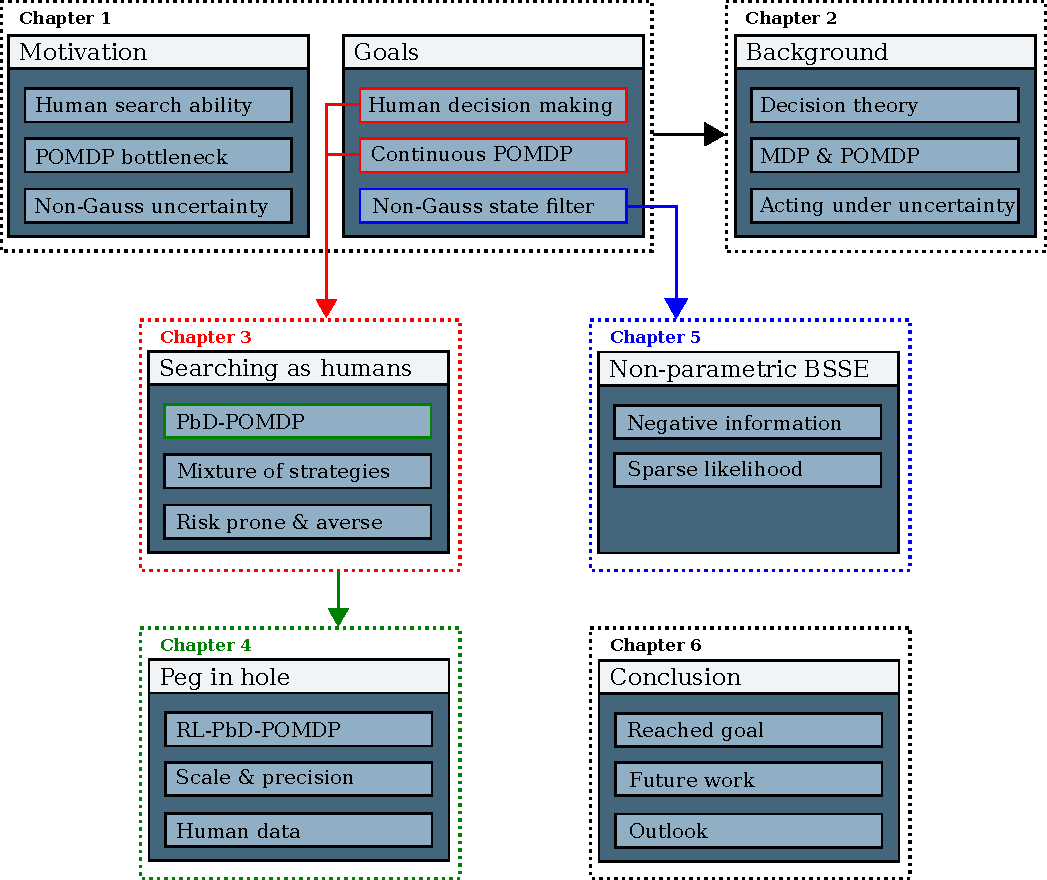
\includegraphics[width=\textwidth]{./ch1-Introduction/Figures/roadmap.pdf}
  \caption{Roadmap of the Thesis with key points. }
  \label{fig:rmap_thesis}
\end{figure}

\section{Thesis outline}

The thesis is structured according to three main contributions outlined in the previous section, 
each comprising a chapter and the following paragraphs give a detailed outline of the structure 
of this thesis, see Figure \ref{fig:rmap_thesis}.

\begin{minipage}[c]{0.9\textwidth}
\paragraph{Chapter 2 - Background}\\
In this chapter we introduce and mathematically formalise the sequential decision making problem 
under uncertainty and we provide a detailed literature review of the related work in this domain.
We provide a brief introduction to \textit{Decision Theory} before focusing on the work 
in AI \& robotics relevant to POMDPs whilst highlighting their relevance and contribution to our work. 
\end{minipage}

\begin{minipage}[c]{0.9\textwidth}
\paragraph{Chapter 3 - Learning to reason with uncertainty as humans}\\
In this chapter we present an approach for transferring human skills in a blind haptic 
search task to a robot in our PbD-POMDP framework. The belief of the human is represented by a particle filter and 
all subsequent beliefs are inferred from the human's motions acquired via a motion tracking
system. A generative model of the joint belief and actions distribution is learned and used
to reproduce the behaviour on a WAM and KUKA robot in two search tasks. Experimental 
evaluations showed the approach to be superior to greedy opportunistic policies and traditional
path planning algorithms. 
We also provide a review of work related to humans taking decisions under uncertainty 
in spatial navigation and haptic tasks with an emphasis on works which consider diminished or no 
visual information. 
\end{minipage}

\begin{minipage}[c]{0.9\textwidth}
\paragraph{Chapter 4 - Reinforcement learning in belief space}\\

In this chapter we present a similar approach to the one in chapter 3, ``Learning to reason with uncertainty as humans'',
with the difference that we explicitly encode the task through the introduction of a binary objective function and we consider 
a peg-in-hole task under high levels of uncertainty. 
The task requires both high and low levels of precision from the agent to be able to accomplish it, which makes it particularly interesting. 
We demonstrate the importance of initially provided human data as opposed to using data generated from a myopic policy.
We learn a value function approximation of the belief space through locally weighted regression and approximate dynamical 
programming. By combining a PbD approach in this Actor-critic Reinforcement Learning framework, we demonstrate an improvement upon 
a purely statistical controller with nearly no additional cost. We refer to this approach as RL-PbD-POMDP. 
\end{minipage}

\begin{minipage}[c]{0.9\textwidth}
\paragraph{Chapter 5 - Non-parametric Bayesian state space filter}\\
In this chapter we present an approach to perform a state space estimation of a map and agent 
given that there is no direct observation between the landmarks and the agent. 
We demonstrate that by keeping track of the applied measurement functions rather than 
explicitly parametrizing the full joint distribution of the landmarks and agent we can fully reconstruct 
the optimal Bayesian state estimation. The advantage of our approach is that the space complexity is linear as opposed 
to exponential. We validate our approach in 2D search navigation tasks.
We also give an overview of the literature of SLAM and emphasis the position of our filter within it.
\end{minipage}

\begin{minipage}[c]{0.9\textwidth}
\paragraph{Chapter 6 - Conclusion}\\
We conclude by providing a holistic summary of our work and achievements. We draw attention to the current 
open problems and directions for future work in the field of uncertainty and reasoning in Artificial intelligence and robotics.
\end{minipage}







